\section{Electrostatic transduction}

Following the tutorials referenced in the assignment, the electrostatics is
added as follows. An air domain fills the cavity between the comb and the
stator. The whole shuttle is a \emph{domain terminal} at \SI{0}{\volt}, which
also returns its total charge and hence the capacitance. The stator floor and
the fixed-finger walls carry the drive potential $\Vd$. An
\emph{Electromechanical Forces} coupling applies the Maxwell stress to the
solid, and a \emph{Moving Mesh} node (hyperelastic smoothing) deforms the air
mesh with the structure, with roller conditions at the two side openings.
Figure~\ref{fig:pot} shows the potential at $\Vd=\SI{50}{\volt}$: the drop
concentrates in the 40 flank gaps and in the two \SI{1}{\micro\meter} tip
gaps of each finger.

\begin{figure}[H]
\centering
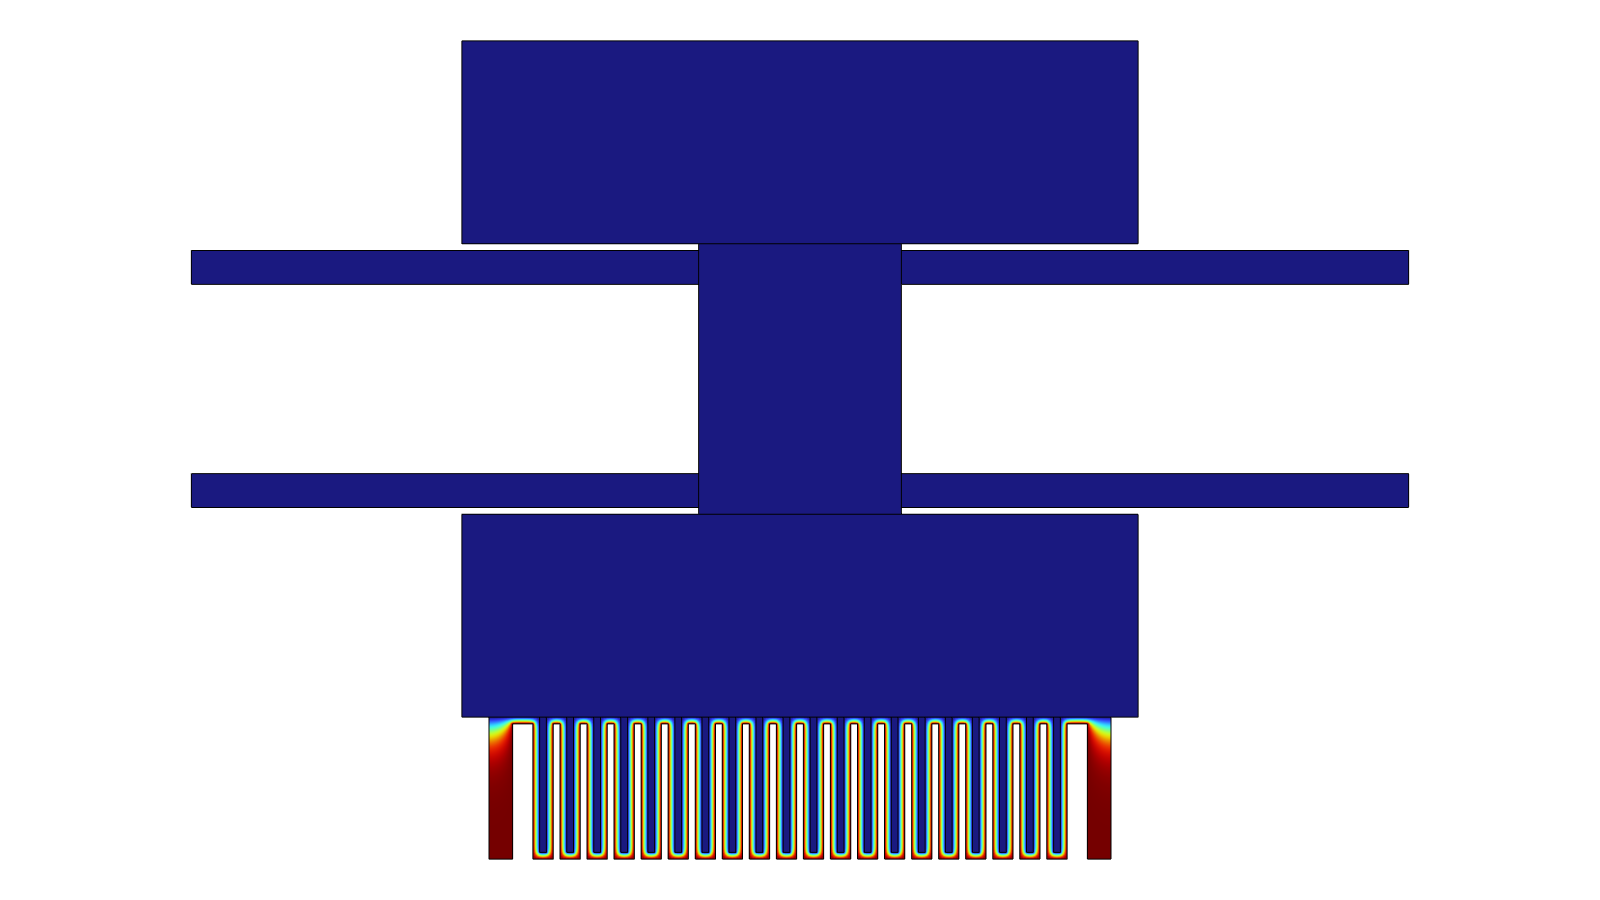
\includegraphics[width=0.8\textwidth]{figures/diag_potential_50V.png}
\caption{Electric potential at $\Vd=\SI{50}{\volt}$. Blue: shuttle terminal
at \SI{0}{\volt}; red: stator and fixed fingers at $\Vd$. The wide end
fingers ($3W_{c}$) are visible at both edges of the comb.}
\label{fig:pot}
\end{figure}

\subsection*{Q4a -- Displacement versus voltage, 0--150 V}

A stationary study sweeps $\Vd$ from 0 to \SI{150}{\volt} in \SI{10}{\volt}
steps, each solution continuing from the previous one.
Figure~\ref{fig:q4a} plots the FEM displacement together with the Part~1
prediction $x=V^{2}N\epsilon_{0}t/(2kh)$.

\begin{figure}[H]
\centering
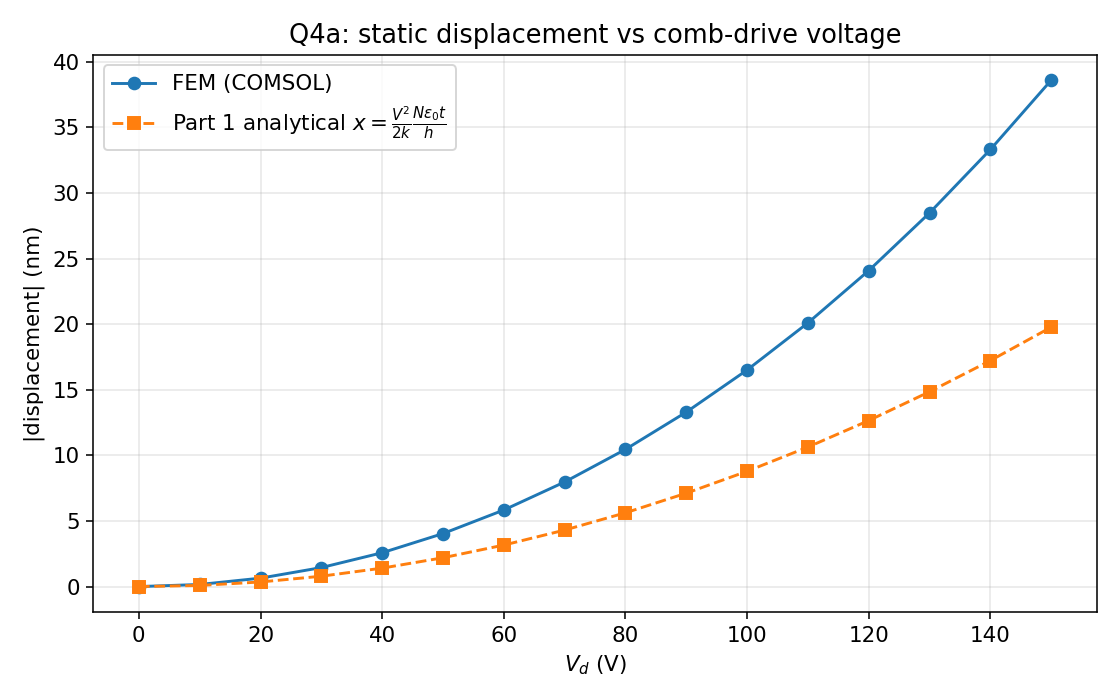
\includegraphics[width=0.78\textwidth]{figures/q4a_displacement_vs_voltage.png}
\caption{Static displacement of the mass versus comb-drive voltage: FEM
(blue) and the Part~1 ideal-comb expression (orange). Both are quadratic in
$V$; the FEM force is larger by a nearly constant factor.}
\label{fig:q4a}
\end{figure}

Both curves are quadratic, but the FEM displacement is $1.84\times$ the
analytical one at \SI{50}{\volt} and $1.95\times$ at \SI{150}{\volt}. The
factor splits cleanly in two:
\begin{itemize}
\item $\times1.09$ from the softer FEM spring (Q1);
\item $\times1.68$ from the electrostatic force gradient. The ideal-comb
  formula counts only the flank capacitance, $dC/dx=N\epsilon_{0}t/h=
  \SI{7.08e-11}{\farad\per\meter}$. In this geometry the comb is engaged to
  $d_{0}=19$ of \SI{20}{\micro\meter}, so two families of
  \SI{1}{\micro\meter} tip gaps remain: mover tips facing the stator floor,
  and fixed-finger tips facing the mass plate. Both close as the shuttle
  moves down and add roughly $\epsilon_{0}W_{c}t/g^{2}$ per tip. The
  force-implied gradient from the FEM at \SI{50}{\volt} is
  $\SI{1.19e-10}{\farad\per\meter}$, i.e.\ the tip gaps contribute almost as
  much force as all the flanks together.
\end{itemize}
The terminal capacitance supports the same picture: $C(0)=\SI{1.51}{\femto\farad}$
against the parallel-plate value $N\epsilon_{0}d_{0}t/h=\SI{1.35}{\femto\farad}$
(the 12\% excess is fringing), and $C$ rises with voltage as the comb engages
deeper. The slow growth of the FEM/analytical ratio with voltage is the
$1/g^{2}$ tip nonlinearity beginning to show -- the same mechanism that ends
in pull-in.

\subsection*{Q4b -- Pull-in voltage}

The voltage is raised in \SI{5}{\volt} continuation steps until the
stationary solver stops converging. Because each step starts from the
previous equilibrium, the solution follows the physical stable branch, and
the first voltage with no stable equilibrium is the pull-in point. The sweep
converges up to \SI{222.2}{\volt} (displacement \SI{94}{\nano\meter}) and
diverges beyond it:
\begin{equation}
  \boxed{\;\VPI^{\mathrm{FEM}} = \SIrange{222}{227}{\volt}\;}
\end{equation}
against \SI{347}{\volt} from the Part~1 tip-gap model
(Fig.~\ref{fig:q4bbranch}).

\begin{figure}[H]
\centering
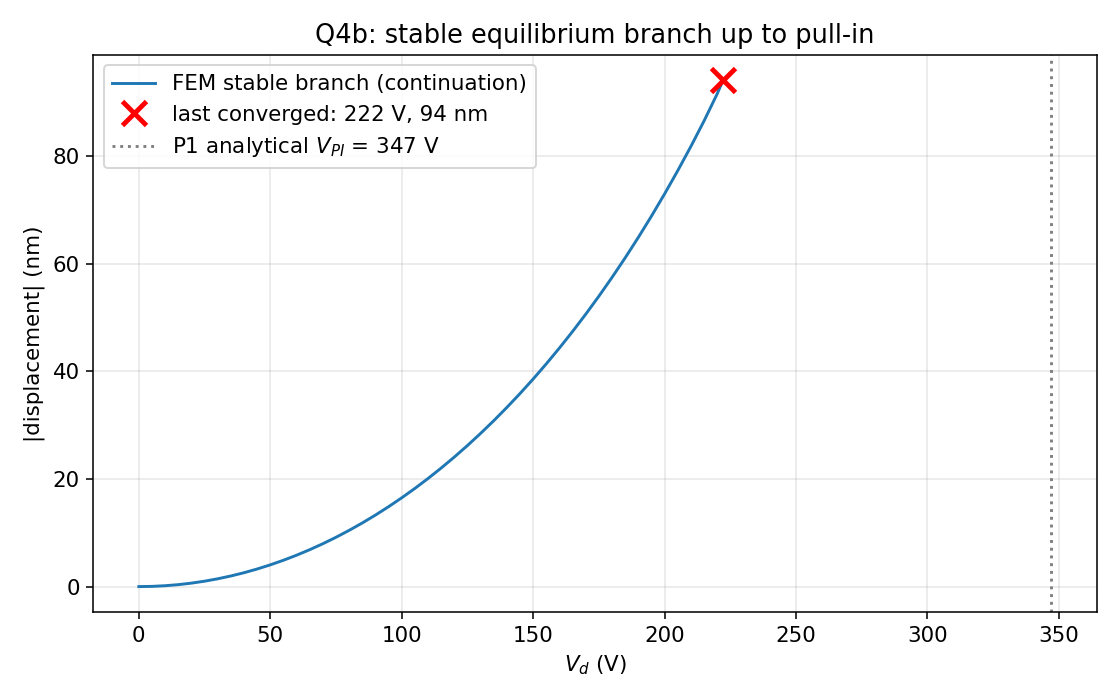
\includegraphics[width=0.74\textwidth]{figures/q4b_vsweep_branch.png}
\caption{Stable equilibrium branch from the continuation sweep. The branch
ends where no stable solution exists; the last converged point is
\SI{222.2}{\volt} at \SI{94}{\nano\meter}.}
\label{fig:q4bbranch}
\end{figure}

Two things stand out: the FEM pull-in is 36\% below the Part~1 value, and it
happens at \SI{94}{\nano\meter}, far short of the $g/3\approx\SI{333}{\nano\meter}$
rule of thumb for a \SI{1}{\micro\meter} gap. Correcting Part~1's formula
with the FEM stiffness and force gradient,
$\VPI\approx347\sqrt{(k_{\mathrm{FEM}}/k_{\mathrm{P1}})\,
[(dC/dx)_{\mathrm{P1}}/(dC/dx)_{\mathrm{FEM}}]}\approx\SI{240}{\volt}$, gets
close to the bracket but still misses what actually happens.

To identify the mechanism, a prestressed eigenfrequency study was run at
increasing bias: stationary solution first, then the eigenproblem linearised
around it. An instability corresponds to an eigenfrequency reaching zero.
Figure~\ref{fig:q4bsoft} shows the normalised stiffness $(f/f_{0})^{2}$ of
the three lowest modes. The axial actuation mode barely softens (it would
reach zero near \SI{445}{\volt}), but \emph{mode 2 -- the rocking mode --
collapses}: \SI{2545}{\kilo\hertz} at rest, \SI{509}{\kilo\hertz} at
\SI{220}{\volt}, with $f_{2}^{2}\to0$ extrapolating to \SI{224}{\volt}. That
matches the observed divergence at \SI{222}{\volt}.

\begin{figure}[H]
\centering
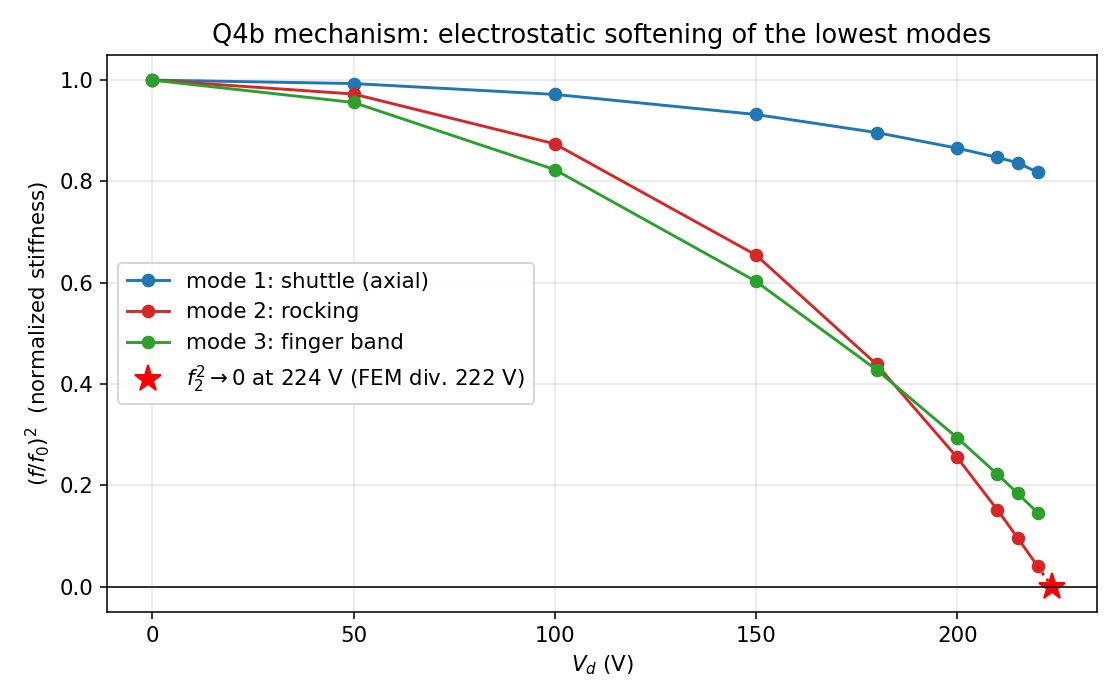
\includegraphics[width=0.74\textwidth]{figures/q4b_eig_softening.png}
\caption{Electrostatic softening of the three lowest modes from the
prestressed eigenfrequency study. The rocking mode (red) reaches zero
stiffness at $\approx\SI{224}{\volt}$, the axial mode (blue) only at
$\approx\SI{445}{\volt}$.}
\label{fig:q4bsoft}
\end{figure}

\begin{figure}[H]
\centering
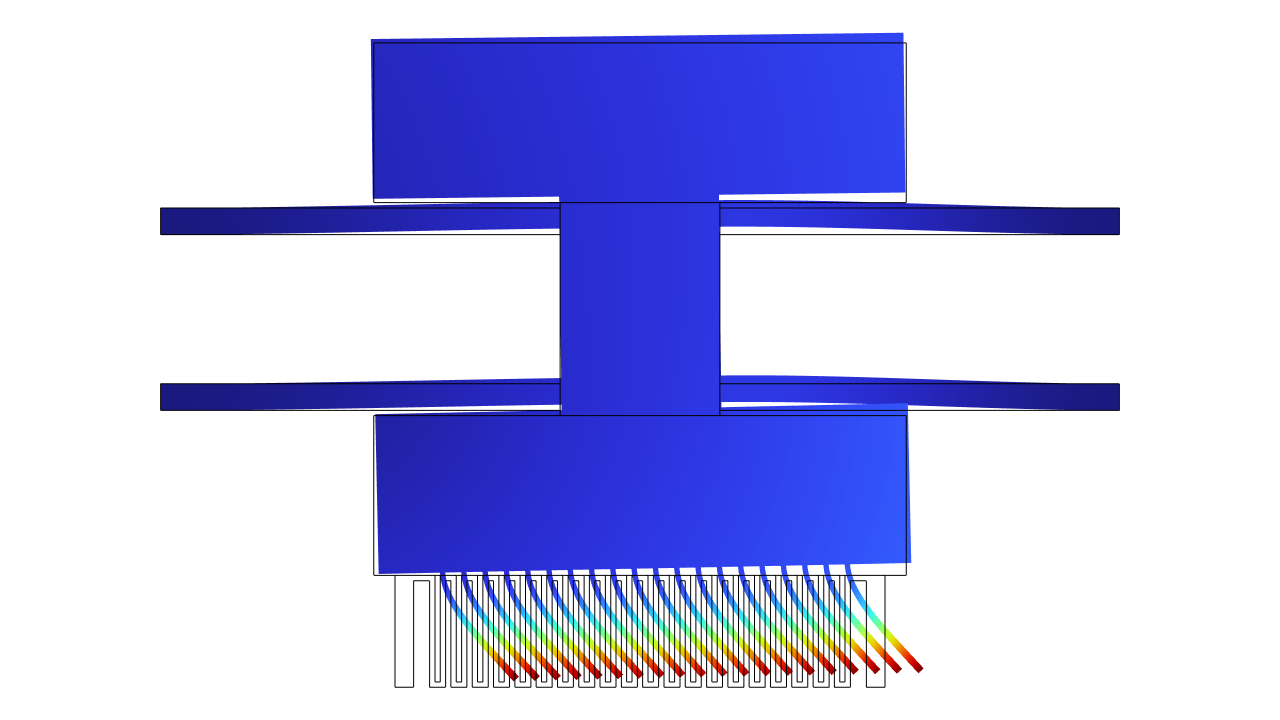
\includegraphics[width=0.74\textwidth]{figures/q4b_critical_mode.png}
\caption{Shape of the critical mode at $\Vd=\SI{220}{\volt}$: a slight
rotation of the shuttle with all comb fingers bending sideways in unison.
This is the mode that goes unstable at pull-in.}
\label{fig:q4bmode}
\end{figure}

The physics is side pull-in. Each finger sits between two
\SI{1}{\micro\meter} gaps, a laterally balanced but unstable arrangement
whose negative stiffness grows as $V^{2}d_{0}/h^{3}$. A small rotation of the
shuttle moves every finger toward one gap wall at once, on long moment arms
(Fig.~\ref{fig:q4bmode}). At \SI{224}{\volt} this rotational softening
overwhelms the suspension. The Part~1 model is a single-DOF axial model; it
cannot represent this failure mode at all, which is why it overpredicts
$\VPI$ by 56\% and also predicts the wrong kind of instability. A design fix
would stiffen the rotation (larger beam separation) or the fingers
themselves (shorter or wider).

A note on method: the assignment suggests the displacement-controlled
continuation from the COMSOL pull-in tutorial (a global equation solving for
the voltage that holds a prescribed displacement). I reproduced that setup --
point probe in the material frame, baseline study with the global equation
disabled, segregated solver groups -- but COMSOL~6.4 fails to assemble freshly
generated solver sequences for global equations that reference the
displacement field (NaN in the moving-mesh residual). The same failure occurs
on COMSOL's own tutorial file when the study is recreated, while the shipped,
older solver sequence runs fine. The voltage-continuation method used above
does not involve a global equation and is unaffected; its bracket is
confirmed independently by the eigenfrequency extrapolation.
